\documentclass[DIV=15,paper=letter,titlepage=true,fontsize=12pt,headings=normal,captions=nooneline]{scrartcl}
\usepackage{Style}
\usepackage[justification=centering]{caption}

\begin{document}
% !TEX root = Main.tex% !TEX root = Main.tex% !TEX root = Main.tex% !TEX root = Main.tex
\begin{center}
{\bfseries\sffamily \textls[150]{Université de Sherbrooke}\\[4pt] \textls[75]{Faculté de génie}\\\textls[75]{Département de génie électrique et de génie informatique}}
\setcounter{page}{0}
\pagenumbering{roman}
\thispagestyle{empty}
\vfill
\textbf{\huge{Rapport d'app7: Space-Invaders}}

\vfill
\textsf{\large Interfaces utilisateurs graphiques}

\vfill
\textsf{Présenté à}\\
\textsf{L'équipe professorale}

\vfill
\vfill
\vfill
\textsf{\footnotesize remis le 12 avril 2024}

\end{center}


\noindent
\rule{\linewidth}{.8pt}

\noindent
Poulin-Bergevin, Charles\hfill Pouc1302\\
Stephenne, Laurent \hfill stel2002\\

\newpage
\renewcommand*\contentsname{Table des Matières}
\tableofcontents
\newpage

\setcounter{page}{0}
\pagenumbering{arabic}

 \section{Mise en Contexte} %\label{Introduction}
 \subsection{Introduction}
 La communication par réseau filaire, et plus spécifiquement coaxiaux, est encore
extrêmenent répandue et essentielle dans plusieurs milieus.
 \FloatBarrier

\section{Reproduction du Problème}
\subsection{Indiquer le schéma électrique}
Nous pouvons voir ci-dessous le schéma électrique de la bobine reçue. Il s'agit d'un réseau en étoile, avec une bobine centrale et trois branches de longueurs variables. La branche B est connectée à un générateur d'ondes carrées de 1 MHz. La branche A est connectée à une résistance de 50ohms. La branche C est un circuit ouvert.

\begin{figure}[H]
    \centering
    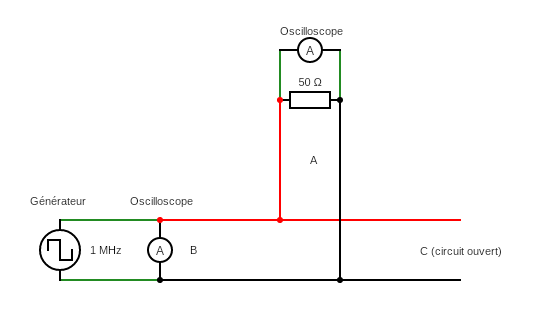
\includegraphics[width=0.7\textwidth]{images/circuit-diagram.png}
    \caption{Schéma électrique du réseau}
    \label{fig:Schema electrique}
\end{figure}

\FloatBarrier
\subsection{Comparer le signal reçu aux spécifications de la carte}
La figure suivante représente l'onde observée lorsque le signal possède une fréquence d'1MHz et qu'un des fils est resté en circuit ouvert. (voir \ref{fig:Signal à 1MHz}) La
ligne bleu représente le signal à l'entrée du circuit (connecteur du fil A). La ligne jaune représente le signal à l'extrémité du circuit
(connecteur du fil B).

\begin{figure}[H]
    \centering
    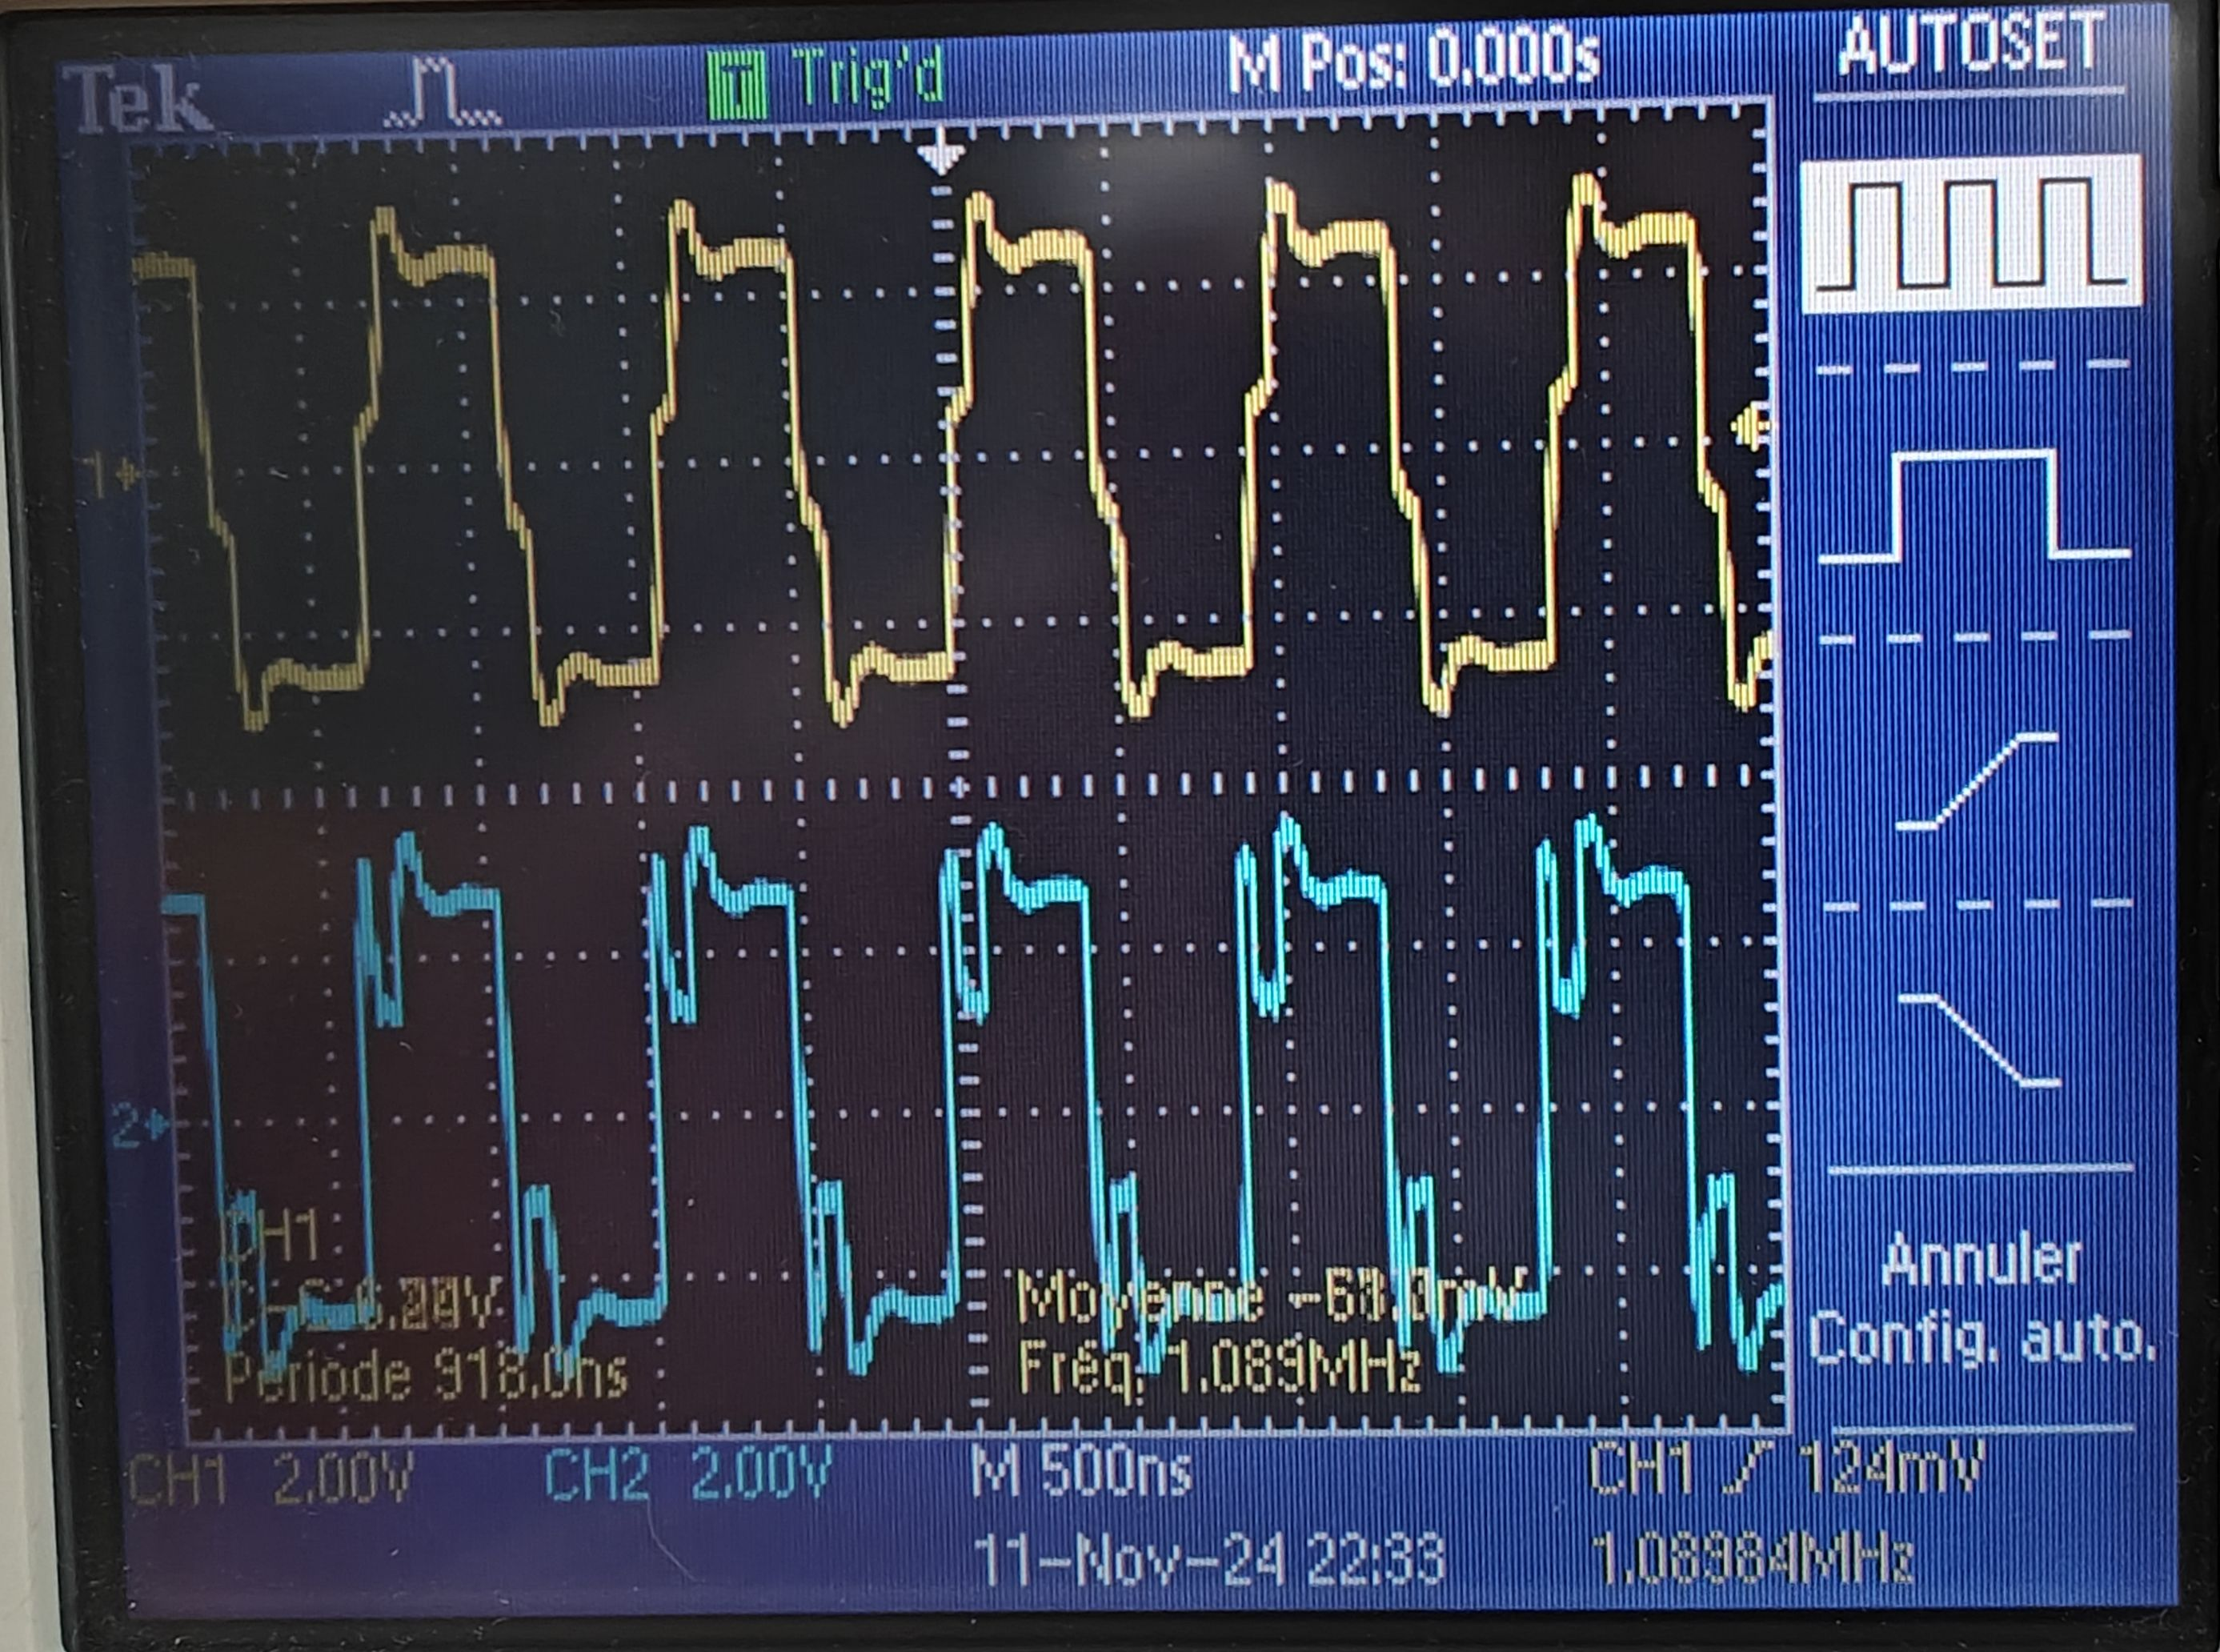
\includegraphics[width=0.7\textwidth]{images/1mhz.jpg}
    \caption{Signaux d'entrée et de sortie à 1MHz}
    \label{fig:Signal à 1MHz}
\end{figure}

On peux voir que les impulsions carrées sont déformées par la réflexion du signal sur la branche ouverte. La réflexion est aussi forte car lorsqu'un fil est laissé en circuit ouvert, sont impédance est infinie. Par contre, les impulsions ont une amplitude de plus de 2V et une durée d'environ 450ns ce qui est adéquat pour que la carte réseau les décode correctement.

\FloatBarrier

\section{Analyse temporelle}
\subsection{Identification de chaque créneau}
En observant la figure précédemment introduite: \ref{fig:Signal à 1MHz}, les conclusions suivantes peuvent être tirées: \\
\\
Lorsque l'on observe le cycle de la ligne bleu, on peut voir que juste après le début de l'émission du signal, une descente se produit lorsque
la réflection du signal se produit et revient à l'entrée du circuit. La réflexion est aussi forte car lorsqu'un fil est laissé en circuit ouvert,
le coefficient de réflection est de 1. On peut observer que la ligne jaune ne semble pas avoir les mêmes "corrections" induites par la réflection
que la ligne bleu. Cela s'explique par le fait que la réflection a l'effet inverse sur la sortie. Si l'on observe attentivement, là où l'onde est
augmenté sur la ligne bleu, elle diminue sur la ligne jaune et vice-versa, mais à une amplitude réduite aussi.

\FloatBarrier
\subsection{Explication du Problème}
 Au niveau fréquentiel, les problèmes survenants sont surtouts liés au principe de l'impédance ramenée. Cela fait, que la réflection crée des annulations
 partielles trop importantes. Cela vient diminuer l'amplitude du signal jusqu'à un point ou la carte ne peut plus lire le signal émis (amplitude
 plus basse que 0.5V). Ce phénomène se produit lorsque la longueur d'un cable est proche d'un multiple de la longeur d'onde du signal.
 Ces problèmes peuvent être rêglés en adaptant l'impédance du circuit (rajouter des fin de connections sur les fils non-utilisés), en s'assurant
 que les fils possèdent une bonne longueur selon la fréquence souhaitée, ou encore en utilisant des cables spécialisés possédants déjà l'impédance
 souhaitée.
\FloatBarrier
\subsection{Mesure par analyse temporelle des branches}
\input{partie-analyse-temporelle/mesure-par-anayse.tex}
\FloatBarrier


\section{Analyse fréquentielle}
\subsection{Explication du problème dans le domaine fréquentiel}
\input{}
\FloatBarrier
\subsection{Détermination précise des longueurs des 3 branches}
\input{}
\FloatBarrier


\section{Solution du problème observé}
\subsection{Solution simple sans modifier le réseau}
\input{}
\FloatBarrier
\subsection{Solution en remplaçant le connecteur en T}
\input{}
\FloatBarrier


\section{Viabilité de la technologie}
\subsection{Problèmes à 1GHz}
\input{}
\FloatBarrier
\subsection{Est-ce qu'un réseau avec des centaines de clients fontcionne en full duplex?}
\input{}
\FloatBarrier


\end{document}